\documentclass{article}
\usepackage{amsmath}
\usepackage{amssymb}
\usepackage{amsbsy}
\usepackage{bbm}
\usepackage{url}
\usepackage{color}
\usepackage{graphicx}
\usepackage{epstopdf}
\usepackage{fancyhdr}
\usepackage{enumerate}
\usepackage{tikz}
\usepackage[ruled,vlined]{algorithm2e}
\usepackage[colorlinks=true,urlcolor=blue]{hyperref}
\usepackage[utf8]{inputenc}

\title{Homework 2}
\author{John Doe, jdoe@stanford.edu}

\newcommand{\Solution}[1]{{\medskip \color{black} \bf $\bigstar$~\sf \textbf{Solution}~$\bigstar$ \sf #1 } \bigskip}

\begin{document}

\maketitle

\section{GCN}
\subsection*{Question 1.1}
\Solution{Write your answer here. \\ Example for writing a matrix $M$: \\
 \[M = 
    \begin{bmatrix}
    1 \ 2   \\
    3 \ 4
    \end{bmatrix}
\]
Example for writing an equation:
\begin{equation}
    F=ma
\end{equation}
Example for inserting a figure: 
\begin{figure}[!htb]
\centering
  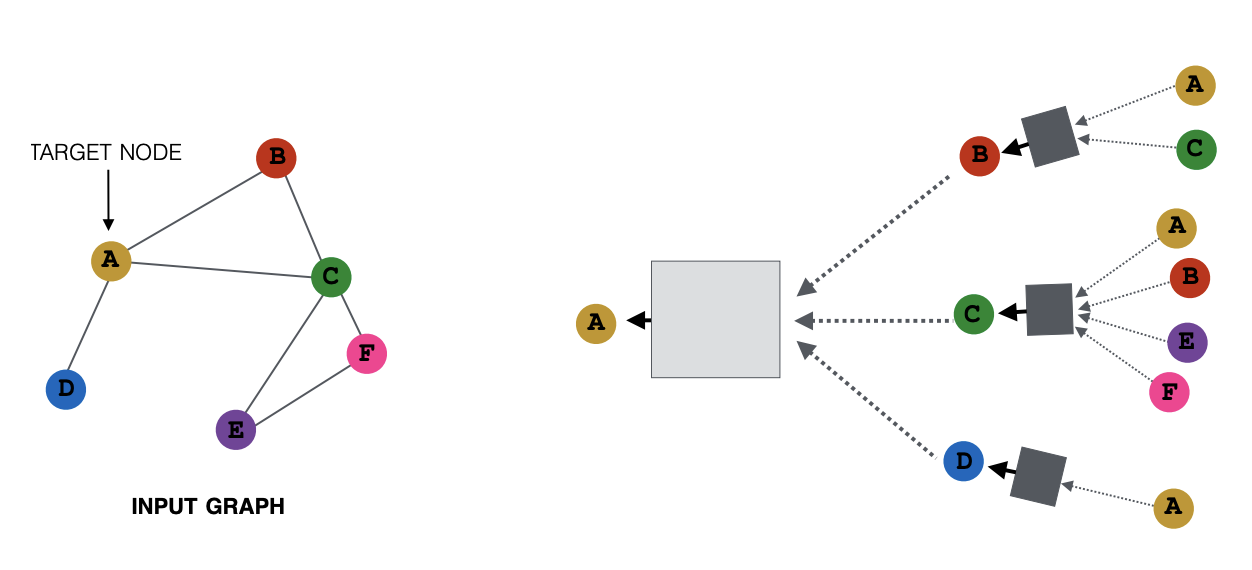
\includegraphics[width=0.8\columnwidth]{Sample_Image.png}
  \label{fig:Q1.1}
\end{figure}
}

\subsection*{Question 1.2}
\Solution{}

\subsection*{Question 1.3}
\Solution{}


\section{Node Embeddings with TransE}

\subsection*{Question 2.1}
\Solution{}

\subsection*{Question 2.2}
\Solution{}

\subsection*{Question 2.3}
\Solution{}

\subsection*{Question 2.4}
\Solution{}


\section{Expressive Power of Knowledge Graph Embeddings}

\subsection*{Question 3.1}
\Solution{}

\subsection*{Question 3.2}
\Solution{}

\subsection*{Question 3.3}
\Solution{}

\section{Honor Code}
(X) I have read and understood Stanford Honor Code before I submitted my work.
\\ $**$ Collaboration: Write down the names \& SUNetIDs of students you collaborated with on Homework 2 (None if you didn’t).$**$
\\ $**$Note: Read our website on our policy about collaboration!$**$







\end{document}
